\chapter{The Size and Shape of Archives}

% In this chapter I will ... 
% FRAME IT compared to news entities

This chapter will take an archaeological approach to digital content, first by analyzing the size and shape of content's containers. Containers include its many representations online---as links, quotes, embeds, and excerpts across search results and social media---and especially the World Wide Web as the Internet's dominant, overarching container. I will begin by defining and contextualizing the modern archive, as well as the word ``archive'' as its possible meanings and definitions have proliferated in the digital age. I will then outline the \emph{layers of containment} that the web exerts on web content, which serve to homogenize content while simultaneously connecting it to a broader ecosystem of media. Finally, I will look at current efforts to store and preserve online content, which each bring their own approaches and limitations to understanding media's history. This chapter will be broad and theoretical in scope, but it serves to frame the issues that journalists and newsrooms face in preserving larger contextual history as well as a news outlet's daily content. I aim to highlight the extraordinary shift in the structure of archives in the digital age. New technologies and institutional pressures have necessitated new methods of storing and saving; archivists have long aimed to fastidiously organize and classify content, but now they can connect content in new ways, complementing the archive's traditional categories and taxonomies with an underlying network.

The digital affords new abilities for \emph{linking} or \emph{networking} the archive, allowing it to dynamically expand, contract, reform, and change shape. In the linked archive, we can forge new connections and create more nuanced context for the information stored inside. Most of today's digital archives and knowledge systems take advantage of some of these new linking features, but they also still inherit many of the limitations of their physical predecessors. Libraries, archives, publishers and others should strive to link and network their archival material.

A linked archive is a collection that: a) treats its contents as an ecosystem of discourses rather than a brittle item to put in boxes; b) actively forms, re-forms, and presents information in more nuanced ways than traditional search; c) gracefully takes in new content and information for future reuse; and d) interfaces with any number of other archives to expand, contract, or reframe its borders. A well-linked archive places context on the same level as content, acknowledging the constantly expanding and shifting shape of research, inquiry and history, and putting the past in full dialogue with the present.

\section{Defining the archive}

The word ``archive'' brings to mind a stuffy room full of closely guarded old books and manuscripts. In the traditional archive or library, books can only be in one place at one time, and always next to the same exact books on the same exact shelf. The atomic unit of information tends to be the book, manuscript, or box of papers, even though each of these contains multitudes of media (text, images, maps, diagrams) and the bibliographies and indexes that offer a window into a book's constituent parts remain limited by space and language. And if your archive dive takes you beyond the scope of the current archive, you'll have to travel to a different one.

But archives come in many forms. More recently, an archive is likely to be digitized, stored on networked servers in databases. Here the archive's stacks and files are virtual, and can be ordered and reordered at will. Books and documents are further atomized and calculable as data. If a search goes beyond the digital archive's scope, it may even be able to reach for information outside of it. ``Archive'' now even turns up as a common verb in digital information management; instead of deleting Google emails, we archive them, which in a sense \emph{de}-organizes it and hides it away. All the same, the message is clear: the email is not gone but archived, saved forever by Google's automatic librarians.

The notion of the archive has changed in both structure and function in the digital age. As both an entity and an action, ``archive'' has perpetually expanding and shifting meanings. Here I will endeavor to define the archive as I will use the term, first by placing it in a lineage of other remediated digital words, then in the context of its use in digital humanities, media archaeology, and software studies.

\subsection{``Thing'' words}

``Archive'' is one of many words that has become increasingly generic and abstract in scope with the introduction of digital media. We often need such generic, all-encompassing words---words that describe a broad swath of things in a very general manner (``things'' being one such word). While reality can be sliced and diced in any number of ways, we sometimes need to talk about the undivided whole. A word like ``thing'' encompasses many words (and actual things) inside it, which can be envisioned as a hierarchy or set of concentric circles around an entity; for example, ordered by levels of abstraction, my tabby cat could be called a tabby, a cat, a mammal, a vertebrate, an organism, or a thing (roughly following Linnaeus' biological taxonomy). This hierarchical structure of language both reflects and shapes the ways in which we have historically classified and organized knowledge, ever since Plato began searching for the ``natural joints'' in reality, and through the most canonical examples: Linnaeus' taxonomy and Dewey's Decimal System.

Today's methods of classifying---and possibly, organizing knowledge in general---have radically changed, and we increasingly need such generic words to describe the digital, ephemeral world around us. The information age has brought us objects, data, documents, information, and content. Its processes include products, services, applications and platforms. Such terms can expand and contract in meaning, and in the process they skirt debate and risk glossing over embedded biases and controversies. They are at the top of a linguistic hierarchy, and threaten to subsume the nuances and contingencies within the subcategories. At the risk of sounding trite, everything is a thing, which is logically impossible to argue (and in fact, the ontology language that underlies the Semantic Web uses ``thing'' as the base layer under which all other words go). But what is a document, or data? How does our use of these words carry contextual weight?

Terms like these are far removed from the realities they describe, and often just as far removed from their original meanings. Remediated words balance an inheritance and a distance from their original (premediated) contexts, and much work has explored the long histories of these terms. Daniel Rosenberg charted the use of the term ``data'' through shifting contexts since the 18\textsuperscript{th} century, noting that it was initially used to describe an indisputable fact or ``given'' in an argument (from Latin \emph{dare}).\autocite[15-40]{rosenberg_data_2013}  Annette Markham likewise questions the use of the word ``data'' in its modern context, suggesting that, ``through its ambiguity, the term can foster a self-perpetuating sensibility that `data' is incontrovertible, something to question the meaning or veracity of, but not the existence of.''\autocite{markham_undermining_2013} Johanna Drucker suggests implementing its counterpart ``capta,'' which highlights the inherently plucked and pre-envisioned nature of all information.\autocite{drucker_humanities_2011}

Other contemporary words have been similarly historicized and questioned. John Seely Brown and Paul Duguid trace the history of the word ``information'' in \emph{The Social Life of Information} and forthcoming research, highlighting its long history as an ``unanalyzed term.''\autocite{brown_social_2002} Likewise, Tarleton Gillespie draws attention to the word ``platform'' in the context of the software industry, focusing on the implications of the term's historical meanings.\autocite{gillespie_politics_2010} ``Platform'' was both an object (e.g. a soapbox) and a concept (e.g. a political platform), and Gillespie sees the word's use in software as borrowing from and conflating these traditional meanings. In each of these cases, the appropriation of abstract words informs and reshapes our own notions of these words and the objects and realities that they represent.

One such remediated word, foundational to the web, is the ``document.'' It was previously understood as a physical, printed record---usually an original. A signed mortgage might be a document, but a photocopy was not; the word ``document'' went hand in hand with the idea of an original. When digital word processing tools co-opted ``document'' as a digital artifact, this made an age-old word new and strange. In many ways, it also forged the foundation of the web, as Tim Berners-Lee used the architecture of the document and file system as the web's basis.\autocite{berners-lee_weaving_2000} Taken for granted today, this decision was not at all a given, and in fact stirred much controversy. Ironically, many of the web's detractors pointed precisely to the web's lack of an ``original'' document copy as its primary shortcoming.\autocites[See, e.g.,][Chapter 18]{lanier_who_2013}{nelson_ted_1999}

\subsection{From archive to database}

The word ``archive'' follows this tradition, but it has exploded even beyond its new digital meaning. Michel Foucault uses the term to refer to ``systems of statements'' that consist of the ``history of ideas,'' the entirety of sayable things and their referents.\autocite[128-129, 137]{foucault_archaeology_1972} Foucault's epistemological archive subsumes both the stuffy room and the digital database into itself. While an archive of books, manuscripts or newspapers is not \emph{the} archive in a Foucauldian sense, the word constantly carries this weight in research and literature about digital history.

Jacques Derrida tracks the origin of the word in his essay ``Archive Fever,'' noting that it comes from the Greek \emph{arkhe}, meaning at once ``commencement'' and ``commandment.''\autocite[9]{derrida_archive_1995} The commencement is the original moment that every act of archiving attempts to capture and return to, while the commandment represents that archive's authority to singularly classify an object and determine its contextual future. Derrida treats Freud's archives as his case study, highlighting the archival moments in the act of archiving itself, and the recursive nature of storage. Here Derrida is working with but complicating Foucault's definition; his archives are more literal, but he still uses the singular ``archive'' to refer to history and its origins.

The \emph{Oxford English Dictionary} defines \emph{archive} as ``A place in which public records or other important historic documents are kept,'' and as ``A historical record or document so preserved,'' while making note of its figurative uses; even this definition implies archives containing archives. The critical and theoretical approaches to archives rely on a reframing of the original term, layering the word with additional meanings and highlighting the philosophical weight associated with collections and stores. So is the archive literal, digital, or figurative? What size and shape does it take? Does it represent an individual's memory, or collective history?

The term shifts based on the \emph{shape} and \emph{scope} of its referent. An archive can be personal, institutional/collective, or universal. Despite the vast difference between, say, a student's bookshelf and the entirety of the World Wide Web, each of these aggregations of information can be figuratively and colloquially considered an archive. Archives morph, connect with, and contain one another. Since the archive evokes all of these scopes and practices, the word expands and contracts in meaning.

An archive always has a border, a point at which the collection stops. It stops on both sides: the \emph{micro} level (what is the smallest unit of information that it indexes---a book, an image, a single letter?) and the \emph{macro} level (what information or metadata does this archive not include?). That an archive has a limit is inevitable, and useful; a limitless archive would be impossible and unhelpful, akin to Borges' exact one-to-one map of the world.\autocite[325]{borges_collected_1999} But ideally, an archive can expand and contract, as needed, on both scales, satisfying both the casual browser and the dedicated researcher. If a researcher asks a question too specific for any one document, the archive could break down the document into its constituent parts; if a user is browsing beyond an archive's boundaries, it might talk to other archives that have the answer. The ideal archive is elastic, polymorphous, and adaptable.

Aside from the borders of archives, there are also borders \emph{in} archives. Traditional, physical archives are divided into sections, stacks and rows, each with dedicated classification schemes that keep books in their right place. Librarians and experts draw and maintain these borders, while others need to speak their language to find their way. Today's digital archives are not so neatly or hierarchically drawn. Derrida uses the border metaphor to describe the recent diffusion of archives: ``the limits, the borders, and the distinctions have been shaken by an earthquake from which no classificational concept and no implementation of the archive can be sheltered.''\autocite[11]{derrida_archive_1995} Claire Waterton, citing Michael Taussig, likewise suggests that the border zone is ``currently expanding, proliferating, becoming permeated by itself.''\autocite[649]{waterton_experimenting_2010} Reflecting the postmodern skepticism towards standard categories and hierarchies, the linked archive reshapes itself into any categorization scheme that a user or collective might define.

These complications make any singular definition of \emph{archive} impossible. Generally speaking, I will use the term to refer to any collection or repository of items that offers interfaces for those items' organization and discovery, with the aim of helping people find information, structure ideas, and do research. This includes the systems surrounding collection itself---organizational, structural, and sociocultural. To put it in Lev Manovich's terms, ``data structures and algorithms are two halves of the ontology of the world according to a computer.''\autocite[84]{manovich_database_1999} I am interested in an archive's data structures (specifically with regard to its items' indexing, metadata, and organizational schemes), as well as its algorithms (the ways to organize, aggregate, repurpose, and present these items to the user).

For my purposes, the ``archive'' is similar to the concept of the ``database'' as considered by Manovich and others. The distinctions between these two terms have been debated extensively, and some scholars have treated traditional, pre-digital archives as databases.\autocite[See, e.g.,][]{manoff_archive_2010,freedman_responses_2007,barnet_pack-rat_2001} I intend to reverse this anachronism, and treat databases as archives. I do this in part to hone my focus onto the collections and systems that provide access to personal, institutional, and historical records for research and inquiry. The archive, unlike the database, pledges perpetual storage, future access and availability. As Marlene Manoff says, ``The notion of the archive is useful in theorizing the digital precisely because it carries within it both the ideal of preserving collective memory and the reality of its impossibility.''\autocite[396]{manoff_archive_2010} Following Jerome McGann's insights, I see the database as a technical instrument used for the structuring and enabling of archives; it is not the archive itself.\autocite[1588]{freedman_responses_2007}

Like McGann and Manoff, I also use the word to emphasize a lineage. Today's information management tools continue to inherit many ideas and techniques from traditional archives and note-taking systems---a fact that ``database'' doesn't emphasize. These systems are always evolving and built atop one another; traces of old technologies are present in current systems. In this sense, many of the applications we use today are systems for organizing and managing personal, institutional, and public archives: search and social media platforms (Google, Twitter), note-taking and citation tools (Evernote, Zotero), content management systems (WordPress, Drupal), ideation and productivity software (Trello, Basecamp), media repositories, codebases, and so on. Archives are also deeply embedded within and linked to one another via APIs, further complicating the picture.\footnote{APIs (Application Programming Interfaces) allow online services to connect to one another for various features and services; one basic example might be a Facebook ``like'' button on a news article.}

The rise of knowledge work has brought more and larger archives, and new computational capabilities have brought a new \emph{kind} of archive with new affordances. We use these archives for both professional and personal ends; whether we read social media and blog posts, create and collaborate on workplace documents, or use data-driven methods to track our health and habits, we are interacting with archives. Jussi Parikka suggests that ``we are all miniarchivists ourselves,'' calling the information society an ``information management society.''\autocite[2]{ernst_archival_2012} Belinda Barnet considers it a ``pack-rat'' mentality, and Derrida succinctly titles the phenomenon ``archive fever.'' Viktor Schoenberger writes that by default, the web saves rather than forgets; this may be the effect, but it misplaces the agency at hand.\autocite{schoenberger_useful_2007} The web stores nothing, while \emph{we} save, store, and sort with abandaon.

%While the following chapters will increasingly hone in on the archives of legacy and digital media publishers, my use of the term here may be broader and slipperier, in order to place the news publishing archive in the context of other archives, and glean lessons from its usual shape and scope. An archive is a collection that is organized for future retrieval and reuse; it is any collection that is not a dump. This encompasses traditional archives, modern databases, and the algorithms and interfaces in between.

\section{The social life of content}

Along with words like archive, document, data, and information, I am interested in the word ``content'' to describe creative works or texts residing on the web. It is a word that is bound to encounter derision, whether from ``content creators'' (never self-defined as such), information theorists or media scholars. In a 2014 talk at MIT, Henry Jenkins referenced the word's derivation from the Latin \emph{contentum}, meaning ``a thing contained.''\autocite{whitacre_podcast:_2014-1} Doc Searls frequently criticizes the term for its ties to marketing, implying a one-way web where content is a catchall term for anything that can be packaged, sold, and consumed online.\autocite{searls_earth_2014}

Another, perhaps friendlier way to describe content is as a ``link.'' When a friend emails you an article, he is less likely to say ``here's a piece of content'' than ``here's a link,'' implying sharing and networking from the outset. Where content implies a container (containment), a link implies a connection (expansion), promising to break free from the contained information. Looking at the link favorably, if a publisher adds a hyperlink to an article, it purports to show not only erudition (the publisher has read and vetted the content within), but also altruism (the publisher is helping the content creator and the user reach one another). But here, the link surrounds the content. In effect, it is the original container, adding the first layer of context to the content, but diluting its core in the process. In studying the origins of the link's structure and the web's infrastructural qualities, we find many ways in which the web's very structure, as well as the creators, indexers, and archivists that work with content, acts as a containing and homogenizing force. The web's simultaneous operations of containment and connection make online media more legible as a networked, aggregated mass rather than a set of distinct and multifarious texts, more often treated with macro-level analyses rather than smaller-scale textual readings.

% Quick note about how this reflects a couple of the link analyses' frameworks for analyzing hyperlink networks; looking at the page, then the URL, then the hyperlinks in the URL, successively

But there is value in honing in on the smaller aspects of online content. A single link accumulates layers of context and connection at each stage of its life on the web. One could view the result as if in concentric circles, as a series of wrappers around the original source. Therefore, the original text (whether itself text, image, video, or a combination thereof) finds itself embedded under several layers of representation. The first such wrapper is the URL (Uniform Resource Locator), which serves to represent multimedia in a homogenous piece of text that renders everything ``uniform.'' From there, several layers of representation are placed on top of it, starting with the hyperlink (an HTML element that forges connections between documents). An HTML document is a hybrid object; links contain links, and content is consecutively embedded in secondary sources, social media platforms, search results and archives. At each stage, the content acquires new metadata created by both individuals and machines, that indelibly affects our understanding of the original source. These varying layers of context and containment reflect new modes of information organization and storage, and ultimately affect the ways in which we organize and represent multimedia works.

\begin{figure}[ht]
\centering
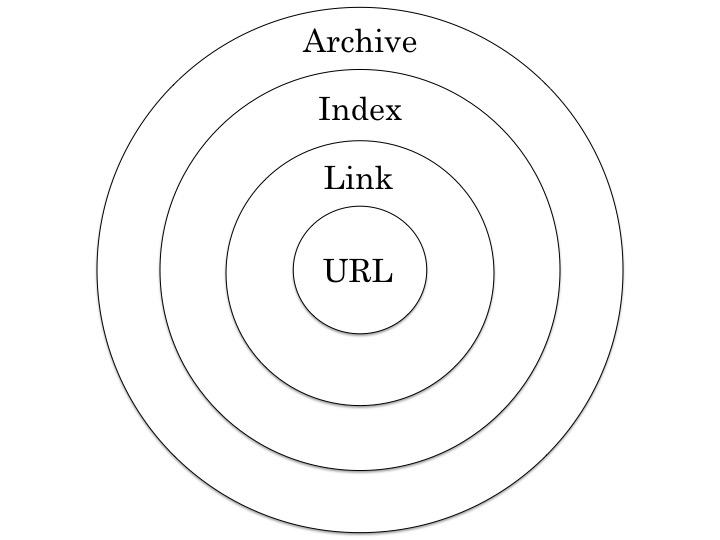
\includegraphics[width=250pt]{figures/layersofcontainment}
\caption{Layers of containment.}
\label{fig:layersofcontainment}
\end{figure}

These stages mark a sort of biography of online content, following Igor Kopytoff's ``biography of things,'' which focuses on the transitional events that mark a thing's history.  Kopytoff complicates the idea of any single, indelible act of categorization on an object---instead, an object is ``classified and reclassified into culturally constituted categories.''\autocite[68]{appadurai_cultural_1986} This especially lends itself to digital content as well due to its ephemerable and duplicable nature; for instance, a Flickr image might turn up in far-reaching corners of the web, activated from archives via various searches. The photo in figure~\ref{fig:fleetweek} lives in eight different Flickr groups and one album, such as ``USN Blue Angels,'' ``Airplanes,'' and ``Curbed SF.''\autocite{joshi_fleet_2014} One user might find it when searching for photos of the Blue Angels (part of the photo's content) or the Golden Gate Bridge (both content and location), while another could simply be searching for photos of fog, or spectacular photos (part of the photo's effect). Still another user could be looking for photos taken on a Canon EOS 7D, or photos with more than 2,000 views. Such categories can be dynamically conceived and created, and digital objects often carry the potential for a nearly limitless number of them.

\begin{figure}[ht]
\centering

\includegraphics[width=375pt]{figures/fleetweek}
\caption{A sample photograph on Flickr. Photo by Bhautik Joshi and used under a Creative Commons license.}
\label{fig:fleetweek}
\end{figure}

The fact that digital objects carry this contextual metadata leads to a detailed history; an old photo of your ancestors won't tell you the exact date, time, and coordinates of its inception, or the camera it was taken on. All the same, that old photo carries a physical trace of reality, a \emph{grain} of history that an archaeologist or forensic investigator might be able to decipher. Meanwhile, a digital object's origins can be forged or erased with relative ease; I could take a screenshot of the Flickr photo and give it a fresh new history, as a completely ``different'' object, claiming that it was taken years earlier, or with a different camera. The ephemerality of digital content and malleability of its metadata leads to many ontological and practical dilemmas; the former is explored by the field of media archaeology, while the latter forms the basis of media search and metadata verification services like Storyful and TinEye. Digital content's history is both abundant and ephemeral, both given and plucked.

A biographical approach to digital content nods both to media archaeology and the contingencies of classification proposed by Kopytoff: ``what we usually refer to as `structure' lies between the heterogeneity of too much splitting and the homogeneity of too much lumping.''\autocite[70]{appadurai_cultural_1986} Digital content lends itself well to these notions of shifting identity. The stock photograph is a rich example of content that is continuously recontextualized; the Blue Angels photo could turn up in a news article about the angels, or about the Golden Gate Bridge, or about the Canon EOS 7D. Its metadata forms its history; at various points of its ``life'' it has been tagged, grouped, searched for, resized, or recolored; some of this history has traveled with it, written by both humans and machines, while some of it was deleted or never captured, now irretrievable. Such a rich social history with myriad possible uses cannot be predicted or summed up by simple, static categories and tags.

Geoffrey Bowker and Susan Leigh Star emphasize the perils of ``splitting and lumping'' in their book \emph{Sorting Things Out: Classification and its Consequences}. Tracing the history of classification as it is used formally (in standards) and informally (in the words, framings and mental models we are perpetually forming), they argue that each act of classification affects the classification system itself, and future classifications in turn. At its most abstract level, classification is the application of language to reality; whether you are calling a kitten ``cute'' or a person ``male,'' you are framing the subject at hand and privileging certain discourses and interpretations over others. Taken at scale, these acts shape our epistemology and understanding of the world. Bowker and Star see infrastructures and standards as intimately interlinked; each one inherits the values and inertias of the systems around it. They point to the 200 standards imposed and enacted when a person sends an email; these standards interact and depend on one another in important ways.\autocite[7]{bowker_sorting_2000} \emph{Sorting Things Out} highlights many of the problems and limits with traditional classification, and suggests frameworks for rendering it more dynamic and responsive.

As such, any attempt to trace an object like a stock photo is also doubling as an analysis of the whole system in place. Content is never just content, and to describe it is also to describe its containers. This notion of embeddedness also points to actor-network theory (ANT) and its treatment of objects and the social interactions around them. Beyond content and people, there is another type of actor in this network too; the search and sorting algorithms run by Google, Facebook or other aggregators and platforms.

\subsection{The URL}

As Tim Berners-Lee tells it, the Uniform Resource Locator, or URL, ``is the most fundamental innovation of the web.''\autocite[39]{berners-lee_weaving_2000} Sometimes called the Uniform Resource Identifier or URI, it allows any address to link directly to any other address simply by pointing to it. But the URL itself is a remediation of old standards and practices. It mimics the file folders on our home computers (an intentional decision, so it could be understood and adopted quickly), implying a hierarchical, document-based structure. Interpreted hierarchically, the URL can be seen as an address, pointing us to increasingly specific locations until we arrive at the document in question. The virtual space of the web here seems to mimic physical space in the world, suggesting that one can find a document down a certain ``path'' under a certain ``domain'' (see Section 3.1). By turning all rich multimedia into ``uniform resources,'' the URL is a homogenizing force, encoding all content as a textual address and turning it into a reference rather than an experience or narrative.

URLs are not created equal, however, and savvy web users can read a great deal of information in this set of text. A ``.org'' top-level domain (TLD), for instance, might imply a nonprofit or philanthropic institution where a ``.com'' connotes a business. A long, seemingly obfuscated URL might contain spyware or viruses. A URL that ends with ``.html'' or ``.jpg'' will probably be a picture, but one that ends with ``/users?friendrequest=true'' is more likely to be telling a social media site to request friendship with another user. Indeed, at the current stage of the web's evolution, a URL is not by definition a resource; it could yield no content and simply trigger a piece of code, allowing any arbitrary action. Moreover, even documents are subject to change, and the web has no built-in way to track content's erasures and additions. In other words, the ``Uniform Resource Locator'' is not necessarily uniform, nor is it necessarily a resource. Even this vague, homogenizing definition does not hold up.

\begin{figure}[ht]
\centering
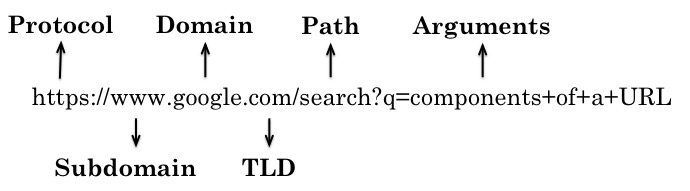
\includegraphics[width=300pt]{figures/annotatedurl}
\caption{Components of a URL.}
\label{fig:annotatedurl}
\end{figure}

Eszter Hargittai points to the need for technical expertise in order to properly understand a URL and the implications behind it.\autocite{hargittai_role_2008} It is easier for a user with less experience with the Internet to be duped by a phony URL that installs spyware or viruses; it is also more difficult for such users to find the content that they need when navigating through links. Further complicating the picture, neither the URL nor the link provide any information concerning motivation or access. In a URL, sensitive documents or paywalled media sites appear the same as free and open information. With the exception of the underlying protocol (``https'' versus ``http''), a URL's overall security or level of access cannot be known without visiting it. Some online publications have constructed paywalls that can easily be ``broken'' through a simple reordering of the URL, or by visiting it from a Google search or a new browser.\autocites[See, e.g.,][]{benton_that_2011}{smith_iv_heres_2015} All of these mechanics and limitations favor information access through technical knowledge, and serve as a barrier to understanding and retrieving information for those who are in the dark.

The URL's fuzzy standards and conventions complicate any overarching attempts to understand or map the web as a whole through its URLs. Many large-scale network analyses of links (discussed at greater length in Chapter 5) rely on URLs to gain insight about the content within, because it is often too technically taxing to gather richer metadata. This is despite the fact that the URL is an arbitrary reference. For instance, an organization might register a site under a variety of domains, or it might register a ``.org'' website despite being a for-profit operation. We're all more likely to trust a ``.com'' or ``.org'' than a ``.biz''---and there's little doubt that Google takes domain names into account when ranking search results.\autocite[See][]{liversidge_whats_2012}

Suffixes like ``.es'', ``.uk'' or ``.tv'' belong to Spain, the United Kingdom and Tuvalu, respectively. Some country-code TLDs restrict domain ownership to citizens of that country, while others are available to all---for a price. These varying practices make it difficult to uniformly map international communication networks by analyzing the link flows between TLDs; for instance, between Brazil and Germany, or between developing countries and Western hubs.\autocites[See, e.g.,][]{chung_inferring_2013}{fragoso_understanding_2011}{himelboim_international_2010} This is in part because it is relatively easy to do such analyses at a large scale, where all you need is a list of URLs and pointers. But the URL is not so easily mapped. The ``.tv'' domain, for instance, was sold by the small Polynesian nation Tuvalu to a Verisign company; Tuvalu maintains a 20 percent stake and a \$1-million quarterly payout.\autocite{cave_i_2000} Hundreds of new generic (non-country affiliated) TLDs are entering the marketplace in 2014-2015, and some, like ``.sucks'' have been blamed for extortion, charging companies as much as \$25,000 per year to protect their brand.\autocite{noguchi_new_2015} Underneath these seemingly simple and technical URLs lie complex commercial and financial transactions.

URL ``shorteners'' such as those employed by the New York-based company bit.ly (whose TLD would otherwise suggest that it comes from Lybia) likewise add additional layers between user and content, and further obfuscate the final destination. With a URL shortener, a small and innocuous domain (such as ``bit.ly/a423e56'') can take a user to any corner of the web, whether at the highest level (think ``google.com'') or its most specific (like ``pbs.twimg.com/media/Bm6QZAGCQAADEOk.png''). Shortened URLs no longer pretend to mimic the spatial world or even most personal computer filesystems; we have replicated and obfuscated the URL to the extent that any sort of uniformity or direction is impossible. Anne Helmond calls this phenomenon the ``algorithmization'' of the link, a retracement of its role from navigational device to analytical instrument.\autocite{helmond_algorithmization_2013}

%Perhaps the explosion of the URL was an inevitable byproduct of the web's very structure. The web is widely distributed and highly networked; it links beyond hierarchical organization schemes like the ``domains'' and ``paths'' of the URL itself. Both Berners-Lee and Theodor Nelson (the original coiner of the term ``hypertext'' and its first champion) explicitly highlighted the power of the link to cut across tree structures and find new, unexpected associations.\autocite[104]{zimmer_renvois_2009} Where knowledge was once shaped like a tree, on the web it looks more like Deleuze and Guattari's rhizome.\autocite{deleuze_thousand_1987}\footnote{figure here too?} As such, one cannot make sense of it using URLs alone. However, links offer a start.

\subsection{The link}

A link is more than just a URL: it wraps the URL in an HTML element that allows it to be quickly accessed from another page, containing additional mechanics and context. Without links, the web would just be a series of disconnected nodes; with links, the web gains edges, and becomes a network.

\begin{figure}[ht]
\centering
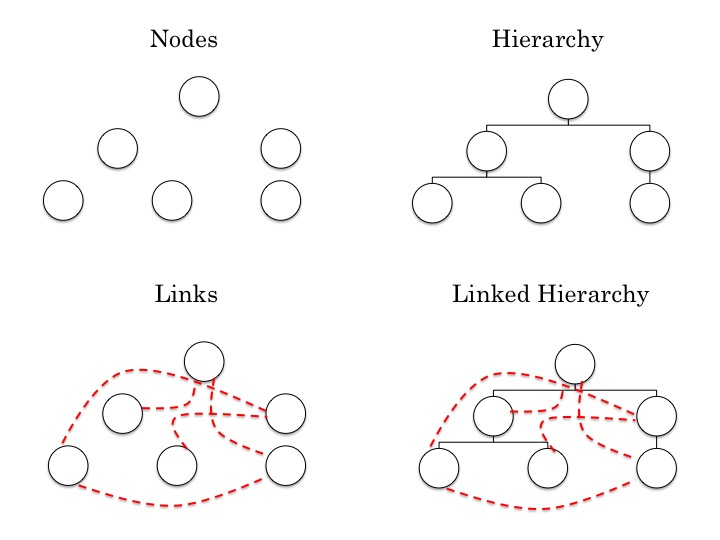
\includegraphics[width=400pt]{figures/linkedhierarchy}
\caption{From nodes to networks.}
\label{fig:linkedhierarchy}
\end{figure}

Bowker and Star suggest that links have the power to classify without any human agency or intervention, and this phenomenon forms the basis of this section: \blockquote{Every link in hypertext creates a category. That is, it reflects some judgment about two or more objects: they are the same, or alike, or functionally linked, or linked as part of an unfolding series.}\autocite[7]{bowker_sorting_2000} The agency shift here is important; the \emph{link} is creating a category, rather than a human actor relying on language. Bowker and Star are not the only ones to cede agency to the link, and many disputes and debates occur over links; even in 2002, Jill Walker asserted that ``links have value and \emph{they give power}.''\autocite{walker_links_2002} In many ways, the link is the battlefield for the political economy of the web, serving as a sort of digital currency and object of value exchange.

All the same, the link is a seemingly innocuous object. We usually consider it taking the form of a blue, underlined piece of text on a webpage (under the hood it is known as an anchor tag---the string ``<a href>\ldots</a>'' and everything in between---in an HTML document). Hovering over the link reveals the true URL behind the blue text. Clicking on the link turns the object into a mechanic, leading a user down a rabbit hole of subsequent destinations and redirects (all employing some dozens of standards) before landing on the target destination---back to the URL. The URL is only one attribute of the link, along with others that determine, for instance, whether to open the link in a new tab or window---so in a literal sense, the link contains the URL.

\begin{figure}[ht]
\centering
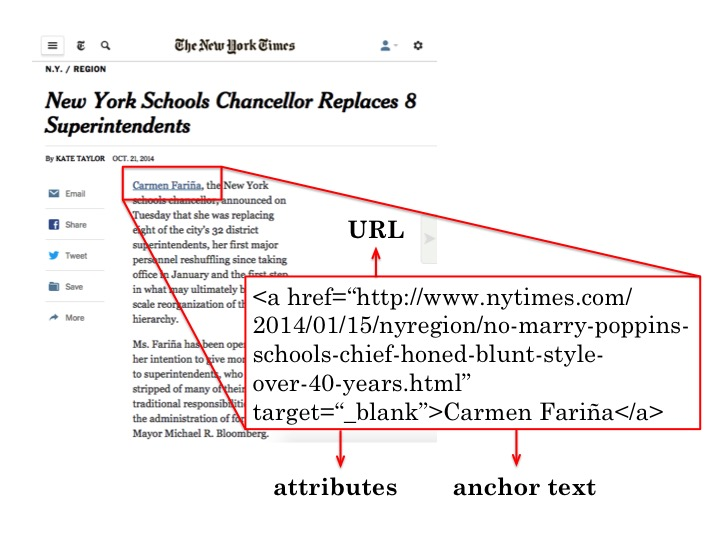
\includegraphics[width=300pt]{figures/annotatedlink}
\caption{Components of a link.}
\label{fig:annotatedlink}
\end{figure}

The link is forever associated with (and perhaps plagued by) the footnote. Theodor Nelson's hypertext manifesto \emph{Computer Lib/Dream Machines} praises the screen for permitting ``footnotes on footnotes on footnotes,''\autocite[DM19]{nelson_computer_1974} and Berners-Lee's web takes the traditional citation as inspiration. Nelson belies himself by consistently contrasting hyperlinks with footnotes; in some senses, one cannot escape being a remediation of the other. But the link's readable text---its manifestation in a browser, known as the anchor text---adds another layer of semiotic containment and enrichment to the original content. The ``jumpable interconnections'' that Nelson envisions are built into the fabric of the writing rather than set aside like a footnote.

Like any sign, the anchor text has no innate relationship to its target. The many flexible uses of the hyperlink emerge at different semiotic layers; when a link says ``click here'' as opposed simply linking the text, it may be forming an indexical rather than symbolic relationship to the target. When a link's text is identical to its address, like ``http://www.google.com,'' it purports to be more transparent, but there is nothing stopping someone from putting a completely different address into the anchor text. This disconnect between anchor text and target facilitates online behaviors both nefarious and playful, ranging from email phishing scams to ``rickrolling.''\footnote{``Rickrolling'' is an online meme wherein an internet user purports to send another person a relevant link, but it redirects instead to Rick Astley's 1987 hit song ``Never Gonna Give You Up.''}

Many studies have attempted to glean insight from the link by assuming, like Bowker and Star, that links create categories. On one hand, it seems extremely liberating to sidestep the ontological dilemma of what that category \emph{is}, and simply treat it as a raw signal. I see this ability as the basis for much of the revolutionary rhetoric of the web and the power of networks. This also forms the basis of link-oriented archival practices that I will discuss further in Section 5.1. % Any Barabasi quote about homogenizing or linking here?
On the other hand, the lack of relation between text and target seems to point to problems with this approach: a sign is not the same thing as a signal. While some search engines and classifiers analyze textual aspects of a link (such as its anchor text, or the surrounding text in the same paragraph or post), few large-scale studies take the text into account or treat linking within a semiotic framework.

The link and its anchor text are increasingly used as a creative textual device amongst journalists, who are continuing to discover its uses. This may be best exemplified by aggregators and email newsletters, which often summarize a larger topic or debate while seamlessly incorporating hyperlinks for attribution, context, and humor. Hyperlink usage may be changing too because of the increase in online literacy; the hyperlink is part of the language of the web, which users understand more and more. The default mechanic of the hyperlink has changed from a full-page refresh to opening a new tab, facilitating a new form of linking ``behind'' rather than ``in front of'' the source text. These creative and technical advances are informed by one another, and a longitudinal study of anchor text usage would help to determine the dynamic evolution of linking practices.

% Should all of this move to the "feed/index" section?
Instead, most studies simply take an aggregate view of link sharing, treating each connection as equal regardless of context. With rare exceptions (such as the ``nofollow'' attribute, which tells Google's crawlers not to follow the link), anyone who shares an article inevitably, and perhaps inadvertently, raises the article's profile and algorithmic rank. Algorithms might therefore prefer controversial links rather than universally liked, substantial, or thought-provoking ones. This could create incentives for publishers to use unnecessarily inflammatory or partisan language, with the assumption that despite how users feel about the content, they will certainly click on it, and possibly share it. Mark Coddington places a cultural studies frame around this phenomenon, where even negative linking implicitly defines the source ``as part of the text's preferred reading.''\autocite{coddington_building_2012} However, some tech-savvy users have adopted techniques like ``subtweeting'' and screenshots of text to avoid easy detection; scholars like Zeynep Tufekci and Helen Nissenbaum have written about such intentional obfuscation, especially in the context of political upheaval and surveillance.\autocites{tufekci_big_2014}{zuckerman_helen_2014}

The many cultural and contextual nuances behind a link or reference are too complex for a computer to discern. This limitation is apparent to Berners-Lee, who has in recent years championed the Semantic Web as a way to make the web more structured and machine-readable. The Semantic Web allows for links themselves to be annotated and queried, so that, for example, we could search for ``users who disagreed with this article'' and not just ``users who linked to this article.''This carries great promise not only for a machine-readable web but a new order of linkage and network formation. The W3C (the standards organization for the web) maintains appropriately revolutionary rhetoric around the Semantic Web, and has tried out scores of marketing terms in its efforts. It alternately envisions a ``web of data'' (rather than documents), a ``Giant Global Graph,'' and ``Web 3.0,'' a particularly telling attempt to couch the Semantic Web as the inevitable next step of forward progress. However, while linked data has been useful in smaller-scale initiatives, the Semantic Web movement has progressed very slowly. It also brings its own problems; while a web of documents is one level removed from the data itself (and therefore more difficult for machines to read), at least it keeps the source context intact. The Semantic Web also forces users to choose particular sets of ontologies, hierarchies and categorization schemes.

Another alternative to the web's form of linkage comes from Ted Nelson, a longtime critic of the web's architecture, whom I will discuss at greater length in the following chapter. As the original hypertext visionary, his scheme, called Project Xanadu, floundered for decades, and has never truly been built in the way that he envisioned. When critics suggested that Xanadu was the first failed web, Nelson bristled: ``HTML is precisely what we were trying to PREVENT---ever-breaking links, links going outward only, quotes you can't follow to their origins, no version management, no rights management.''\autocite{nelson_ted_1999} Xanadu's most important feature, absent from the web, is the two-way link; when one document referenced another, the target document referred back to the original in turn. The hyperlink on the web, for all its flexibility, does not escape the trappings of the footnote in this single, very important way. Like footnotes, links always move backward, and given the lack of a canonical URL on the web (another of its limitations, which the URL-shortening phenomenon compounds), finding all the citations for a single document is next to impossible. The NewsLynx project has documented its challenges in doing just that, while Jaron Lanier believes this simple omission has profoundly affected culture and economics, which forms a cornerstone of his 2013 book \emph{Who Owns the Future?}\autocites[Ch. 18]{lanier_who_2013}{abelson_hyper-compensation:_2014}

But in the absence of replacing or reconfiguring the web's current structure, the one-way, semantically meaningless link remains the web's primary organizational scheme, and the ``click'' remains the proxy for attention and engagement. Clicking on a link is not only a navigational mechanic; it is a signal of intent and interest, which influences algorithmic decisions and other readers in turn. It is also often a financial transaction between unseen actors; each link clicked and page viewed is a new ``impression,'' causing money to change hands between content distributors and advertisers. This has in turn changed the aforementioned semiotics of the link, and the meaning of its anchor text.

For instance, there has been much controversy surrounding the news headline in the hyperlinked age. Consider a story about the foundations that support tuberculosis research. Where a traditional headline might read ``The Global Fight Against Tuberculosis,'' a more recent one is more apt to say, ``It Kills 3 People a Minute, but That's Not Stopping This Group of Heroes.''\autocite{karsch_it_2014} The headline is colloquially known as ``click bait,'' playing to a user's innate curiosity (Atlantic writer Derek Thompson calls it the ``curiosity gap'')\autocite{thompson_upworthy:_2013} without telling them the substance of the article or the actors in play (tuberculosis, the victims affected, the Global Fund, the Gates Foundation, and others). These actors and the issues they are tackling are reduced to pronouns. Here even the content becomes glossed, and a click is likely to signify curiosity about what the content \emph{is}, rather than any genuine interest in the content itself. Machines are not likely to recognize these nuances, which results in false identification of public interest and discourse. Upworthy's organizational structure is telling; the company creates no original content, but instead employs people to trawl the web, find content, and repackage it with a new headline. Upworthy has built a valuable business not by creating new content, but new containers.

\subsection{The feed, the index}

Links rarely exist in isolation, and one form that the link often takes is as part of a list or sequence. Whether it is a digest (on email), a feed (on Facebook, Twitter, or RSS), a set of search results, or a list of ``related articles,'' users are almost always confronted with several choices for what to click on. In this section, I look at the ways in which links get aggregated, indexed, and fed to users. Indexes and feeds can allow for a higher-level view of a major topic, author, or other organizing factor, but at the expense of hiding the richness of the content within.

The aggregators, indexers, and summarizers of the web are its search engines and social media platforms, run by some of the most powerful and profitable tech companies in the world. While the content creator usually has to win the attention of the distributor, the distributor in turn must always play the aggregator's game. This is evidenced by Upworthy itself, who in December 2013 found its content potentially demoted in Facebook's algorithm with no meaningful explanation, shrinking its immense traffic to half of its previous size.\autocite{carlson_upworthy_2014} Another major content distributor, the lyrics annotation website Rap Genius (now a general annotation and reference site called Genius), found its pages move in December 2013 from the top hit on Google to its seventh page, due to changes in Google's algorithm.\autocite{constine_google_2013} These content aggregators can move around large swaths of content (millions upon millions of interlinked pieces) via slight changes in their codebases, with no obligation to inform anyone of the reasons, or even that it is occurring.

But Google did explain its reasoning for the Rap Genius demotion, and the dispute was telling. Rap Genius had launched a ``Blog Affiliate'' program, which clandestinely offered to tweet out any blog post in return for links back to the Rap Genius site. In other words, Rap Genius was engaging in SEO (Search Engine Optimization) spam, attempting to falsely boost its search rankings by asking bloggers to post unrelated links back to their site. This is one high-profile example of what many smaller players do every day in order to keep their businesses alive: game Google's algorithm in order to bolster their search rankings. SEO is, in effect, an entire industry built on gaming links.

This works because Google's PageRank algorithm is primarily derived from who is linking to whom. Their link-based classification scheme is what made them the dominant information provider that they are today. Google famously published their initial PageRank algorithm, and once the cat was out of the bag, advertisers and spammers began to exploit it, inserting links not for their usefulness or relation to the text, but to improve their pages' search rankings. Moreover, many website hacks and attacks occur merely in order to insert hidden links on the targeted sites. In the process, Google has had to remain one step ahead of the advertisers, with the link as the battlefield, influencing the web and changing its structure in turn. But this battle has mostly been played out by machines, which are responsible for a substantial amount of the links created---as well as the links browsed and followed---on the web. Besides a generic, easily replaceable piece of metadata in a web request, it is extremely difficult to tell whether a website request is coming from a human or a machine.

%Prior to PageRank, web crawlers and indexers like Yahoo, HotBot, and AltaVista provided a plethora of options for Internet search (even these, in all their heterogeneity, were seen at the time as a major threat to the open web). But each was based on a traditional, hierarchical classification scheme. In PageRank, Google found a way to embrace the web's disorder; where Yahoo insisted on keeping an organized system, Google relied on links to sort everything out. Clay Shirky argues that this is what allowed Google to surpass Yahoo and become the first truly ``Web 2.0'' company, asserting that on the web, ``ontology is overrated.''\autocite{shirky_ontology_2005}

% More background here on early link-based schemes for finding content?

In Google's published PageRank paper, Sergey Brin and Larry Page provide a curious ``intuitive justification'' for their algorithm that seems to conflate human and machine: \blockquote{PageRank can be thought of as a model of user behavior. We assume there is a ``random surfer'' who is given a Web page at random and keeps clicking on links, never hitting ``back'' but eventually gets bored and starts on another random page. The probability that the random surfer visits a page is its PageRank.\autocite[110]{brin_anatomy_1998}} This is a very strange user indeed, assumed to be easily ``bored,'' distracted, and clicking on links at random. Moreover, this was an assumed user in 1998, and the ``model of user behavior'' must undoubtedly be changing as the web's capabilities and browsing habits change (and indeed, Google's signals have changed in response, though links remain crucial).

While links are shared for a variety of reasons---some of them more nefarious than others---the blogging and tweeting culture of ``Web 2.0'' holds to the principle of link sharing for mutual interest and benefit. If two bloggers like one another's content, they might agree to link to each other on their respective blogs. This happens on the ``blogroll,'' a list of other blogs that a blogger might recommend, usually presented as links in the blog's sidebar. Social media and blogging sites in particular are places of transactional link exchange, with implicit conventions and expectations beneath each link or like. These link exchanges solidify existing networks of bloggers and content creators, perhaps galvanizing the network but at the risk of collapsing into ``filter bubbles.'' Many studies of links have traced political homophily, public debate, blogs and global flows of information; if we take these at face value and treat hyperlink usage as a proxy for importance, impact, and communication, then link-sharing can turn conversation inward, allowing searchers to see only blogs that have overtly linked to one another (blogs which, presumably, have similar views and opinions).\autocite[See][]{graells-garrido_data_2013} While the web may allow for a more heterogeneous group of voices to surface than in traditional media, one must still take part in link sharing, leading bloggers into already-established and tightly wound networks. This leads to what Philip Napoli refers to as the ``massification'' of the hyperlink: in the editorial and algorithmic decisions that determine where links are placed and directed, there is a distinctive replication of old mass media patterns.\autocite{tsui_hyperlinking_2008}

While content creators, distributors, and aggregators are locked in this battle over links, what happens to the actual user who visits a site, application or search engine? The user is presumably after content, and unless they were provided with a direct URL, they can only access it through this series of layered containers. Moreover, the content may be replicated and embedded in different contexts and myriad places around the web. The end result, when a user goes to Google to search, is often repetition. The same piece of content appears everywhere, such as a canonical image for a popular news story, meme, or theme.

\subsection{The archive}

Online content's final resting place is in the database (or archive), but the context and metadata around a digital object is still subject to perpetual change; any new link, like, click, or download updates its history. Indeed, the four contextual layers that I have offered here, while a theoretically useful framework, belies a more complex lifecycle; sometimes the content actually reaches a database (and is thus archived) before it even has a URL (and is thus accessible).

The database is a different form of container than the others, as it is in fact not truly of the web; it merely talks to it and works with it. Web users increasingly treat the web as a database, but there is no single database; instead there are very many, housed on servers around the world. Each of them faces a similar challenge: how to flatten and store the infinite possible contexts, networks, and signals that the web has created around each piece of content, into a format that allows a user to find it efficiently using any number of contexts. Perhaps a user is looking for everything stored in a specific time frame, a certain format, a dedicated category, or any combination thereof; in each case, the archive serves the role of storing and retrieving the information needed.

The ideal archive would anticipate any possible need from any possible user, whether they request content today or far into the future. Any signal that is left out is lost potential knowledge. So an archivist, most often associated with storing the past, also plays a crucial role in predicting and affecting the future. Derrida calls the archive ``a \emph{pledge}, and like every pledge, a token of the future.''\autocite[18]{derrida_archive_1995}, but there is no reasonable way to store every possible route through a database that a user might take; this would require infinite storage and processing power.

Seen in this way, the database is perhaps the only truly containing force on the web; the prior stages are in fact expanding contexts and meanings for each piece of content, and it is only in retrospect (through the archive) that it becomes contained. However, we cannot see the content \emph{except} through the archive. And with the assumption that a border must be drawn through the expansive, innately borderless web, the question is where and how to draw it. Lisa Gitelman laments the way in which the archive reduces ``ideas into character strings,'' or in the case of rich multimedia, encoded, flattened and unsearchable bits.\autocite{gitelman_response_2013} Character strings and encoded bits are devoid of context and semantic meaning. They certainly do little justice to the richness of the original content, which points to a proliferation of associated narratives.

My aim is not to suggest any overarching solution to the limitations of the archive; as I will discuss in the following chapter, it is this very impulse that has often set back the work of retaining knowledge and history. Bowker and Star point to the myriad efforts of ``universal classification,'' dating back to the Tower of Babel, all of which have essentially failed. In order to fully recognize and remember this, they suggest the framework of ``boundary infrastructures'' to acknowledge and work with the limitations of traditional classification. Boundary infrastructures make use of boundary objects: ``those objects that both inhabit several communities of practice and satisfy the informational requirements of each of them.''\autocite[297]{bowker_sorting_2000} In practice, these objects (and the infrastructures that work with them) will maintain slightly different meanings in each community, but they are common enough to be recognizable to multiples. Boundary infrastructures emerge as more of a framework than a solution, but they rightly discourage the drive for an overarching schema for every object and community. By recognizing that no system will ever be perfect, it instead highlights the need for a loosely linked multiplicity of them. Such a framework can help when considering the structure of any archival endeavor.

Likewise, the web itself should not be universally schematized, and its content will never be singly and correctly categorized. In a sense, the proliferation of databases and motives for classification that the web provides allows for more ``ways in'' to the content than if the web were stored at a single endpoint. %cite weinberger here?
The Semantic Web is an interesting hybrid of universal centralization and networked distribution; it aims to bridge traditional taxonomy and contemporary chaos through its use of user-generated ontologies. In order for machines to understand a network, everything must be definitively categorized, but the categorization scheme itself is subject to change. Certain standards arise, but each individual or community is free to create its own form of linked data. This has allowed certain communities, most notably the medical industry, to make great use of it; if a 50-year-old smoker is complaining about shortness of breath and a fever, a doctor can ask a linked database for all diagnoses of similar patients. Linked data has also been a factor in the news industry, with many media publishers connecting to OpenCalais or \emph{The New  York Times}' Semantic API for added context. But linked data on the web has proven difficult, and the slow adoption of the Semantic Web may have to do with its reliance on ontologies. Even if multiple ontologies can coexist, they are still trying to compromise the web's inherent disorder.

%Archive fever is both a personal and an institutional drive. Google and Facebook store user data (including user-created content) with abandon, inventing new contexts at each turn. Users bookmark, download, pin, and clip online resources, sometimes all at once. Built-in browser solutions like bookmarks and history haven't changed their structure in years, and it shows---they store nothing but the URL. ``Bookmark'' is a misnomer of a remediated word, as books can't change or disappear overnight, while ``history'' implies a time machine that the web doesn't have. Personal note-taking and online ``snapshot'' tools aim to create a sort of personal, annotatable intranet for users that want to filter signal from the noise (see applications like Evernote, Pinterest and Zotero). However, aside from folders and tags, none of these systems provide a useful way to store meaningful associations between these documents.

%The associations, trails, and lists sparked by the web add to the possible avenues for research; the myriad interconnections between documents may be more responsible than anything else for the seemingly unprecedented amount of information in the information society. In response to this, as well as the web's innate ephemerality, users store everything.

\subsection{Erasure and afterlife}

Content has an afterlife when it is reactivated from the archive at a client's request. Some content stays dormant indefinitely: nearly one-third of all reports on the World Bank's website have never once been downloaded.\autocite{trevino_which_2014} While this may seem dire, it is not to say that the knowledge contained in the World Bank's documents has been utterly forgotten. The document could be distributed at another URL, or by email, or presented at a conference---the inability to track it is part of the problem. But the information is not helpful in the current format. If the World Bank's PDFs are lying dormant, they might consider using HTML, adding links and references from around the web, repackaging and remixing the data, or inviting user comments. All of these variations and annotations could help to unlock and link their data and insights.

But some content may be worthless, misleading, slanderous, detrimental, embarrassing, or outright false. Whether it's an outdated scientific fact, a politician's off-color comment, or a teen's suggestive selfie, not everything should be stored and remembered forever, as-is, without context. Samuel Arbesman's \emph{The Half-life of Facts} emphasizes the drift in knowledge over time, reminding us that information requires constant care and upkeep to remain useful (not to mention maintaining privacy, legality, and security).\autocite{arbesman_half-life_2013} But how should such context be presented, and who should decide or control what is saved and stored? And how can one control a digital object's history and context after it has been replicated and remixed around the web?

Our personal and institutional archive fevers are, in some ways, understandable. Content changes and disappears on the web all the time. The web is an ephemeral stream, and you won't step into the same one twice; Barnet equates web surfing with ``channel surfing.''\autocite[217]{barnet_pack-rat_2001} As users, we know the phenomenon as the dreaded \texttt{404 NOT FOUND}. Researchers led by Jonathan Zittrain found that 30-50\% of links in scholarly papers and legal opinions no longer work (a phenomenon known as ``link rot''), and even when they work there's no telling how much they have changed since being cited (this is ``reference rot'').\autocite{zittrain_perma:_2013} The Hiberlink project has been researching reference rot in scholarly articles, finding that as many as 70\% of linked web pages were irretrievable in the form they were originally cited.\autocite{_one_2015} Similarly, the NewsDiffs project discovered that the average breaking news story is edited and updated several times at the same URL; out of 28,000 New York Times articles, they found 44\% that had changed at least once, and only one in four of these changes lead to official corrections.\autocite{lee_version_2013}

To combat link rot, Zittrain leads the Amber project, which supports a ``mirror as you link'' approach: for instance, if a blogger links to another site, Amber downloads the linked page directly to the blogger's site.\autocite[See http://amberlink.org; see also][]{zittrain_fourth_2010} This petrifies the document, freezing it at the time that it was cited, and offers a fallback in case the link disappears or changes. This approach can be expanded by ``spidering'' out to the links of the target document in turn. Spidering is the default mode of computer browsing; this is how Google's random surfer surfs, and how the Internet Archive saves, always limited by the structure of the link network. Meanwhile, the Archive Team aims to preserve discussion forums and old blogs. The Library of Congress saves websites by manually choosing them, often taking an ``aggregate the aggregators'' approach and storing large text databases, such as Project Gutenberg and Twitter.

% Another complicating layer: digital archiving projects (e.g. Internet Archive) "take the website as the main unit of archiving (Brugger 2012) and privilege the content of a website over its socio-technical context. (Weltevrede 2009).  The website as an archived object is favored over other natively digital objects where the website is archived over “the references contained therein (hyperlinks), the systems that delivered them (engines), the ecology in which they may or may not thrive (the sphere) and the related pages, profiles and status updates on platforms” (Rogers 2013). Thus, in the archiving process the website is detached from the larger web context it resides in." (Helmond 2013 MIT8). This means even networking the digital archive has its limitations and challenges; where do you start/stop linking?
% Also see Brugger "When the Present Web is Later the Past" and "Website history and the website as an object of study"

% Also BuzzFeed deleting its history, U.S. News relying on LexisNexis

Most of these endeavors are publicly or institutionally funded, but the case of Twitter brings up the role of media and technology companies in archiving and organizing our history. In a 2014 talk at MIT, Tarleton Gillespie emphasized the responsibilities that companies like Google, Facebook, and Twitter have towards the contemporary public sphere, global information flow, and implicitly, history.\autocite{whitacre_podcast:_2014} But even public and nonprofit efforts often come under scrutiny, as the Library of Congress' technology efforts were recently criticized for ``digital neglect,'' and the Internet Archive has been accused of preserving ``a specific set of values, a perspective,'' as limited and opinionated in its worldview as any traditional archive.\autocites{the_editorial_board_digital_2015}{abreu_collection_2015}

Most link preservation efforts primarily rely on repeated mirroring, or copying---as the Stanford University Libraries' LOCKSS program acronym says, ``Lots of Copies Keep Stuff Safe.''\autocite[2778]{zittrain_fourth_2010} Whether or not it keeps stuff safe, lots of copies might keep stuff from being organized and traceable. While I will treat the historical implications of copying in the next chapter, Marlene Manoff implicitly attributes archive fever to the sheer ease of copying; if a user were in an actual archive she wouldn't scan every page, but she is happy to save and even re-host an entire database with just a few clicks.\autocite[386]{manoff_archive_2010} This creates an arbitrary number of digital replicas online and explodes the notion of a ``canonical'' version at a specific URL.
%\footnote{(possible figure here with layers of containment/petrification of a document: scanned PDF, image, digital pdf, html doc)}

In this chapter, I have aimed to broaden the scope and meaning of the word ``archive'' to encompass digital databases and personal note-taking systems alike. I have considered the web-as-archive in order to highlight the ways in which the web exerts influence as a particular type of archive and network, with its own blend of data structures and algorithms. The paradox of the online archive lies in the ways it both contains and links documents. It contains them in a traditional sense, reducing media to addresses, representations, and signs. But it another sense the new order of archive connects media, by highlighting each artifact's role in a broader network or ecosystem, with new potential paradigms for organization and reuse.
